% !TeX spellcheck = de_CH
%%%%%%%%%%%%%%%%%%%%%%%%%%%%%%%%%%%%%%%%%%%%%%%%%%%%%%%%%%%%%%%%%
%  _____   ____  _____                                          %
% |_   _| /  __||  __ \    Institute of Computitional Physics   %
%   | |  |  /   | |__) |   Zuercher Hochschule Winterthur       %
%   | |  | (    |  ___/    (University of Applied Sciences)     %
%  _| |_ |  \__ | |        8401 Winterthur, Switzerland         %
% |_____| \____||_|                                             %
%%%%%%%%%%%%%%%%%%%%%%%%%%%%%%%%%%%%%%%%%%%%%%%%%%%%%%%%%%%%%%%%%
%
% Project     : BA Welti Keller
% Title       : 
% File        : tests.tex Rev. 00
% Date        : 16.12.2014
% Author      : Tobias Welti
%
%%%%%%%%%%%%%%%%%%%%%%%%%%%%%%%%%%%%%%%%%%%%%%%%%%%%%%%%%%%%%%%%%


\chapter{Tests}\label{chap.tests}

Dieses Kapitel listet die Testfälle auf, die zu Beginn des Projekts definiert wurden. Für jeden Testfall sind, wo nötig, Vorbedingungen definiert. Ein Testfall beschreibt Aktionen, die vorgenommen werden müssen sowie das zu erreichende Resultat.

Die Testergebnisse sind am Ende jedes Testfalls angegeben.

\section{Testaufbau}
In der Testanlage stehen ein \gls{logger} und drei \glspl{sensoreinh} zur Verfügung. Die \glspl{sensor} sind unter einer Aluminiumplatte montiert, die auf Elastomer gelagert und auf einem Holzgestell verschraubt ist (Abbildungen \ref{fig.testaufbau1} und \ref{fig.testaufbau2}).

\begin{figure}
	\centering
		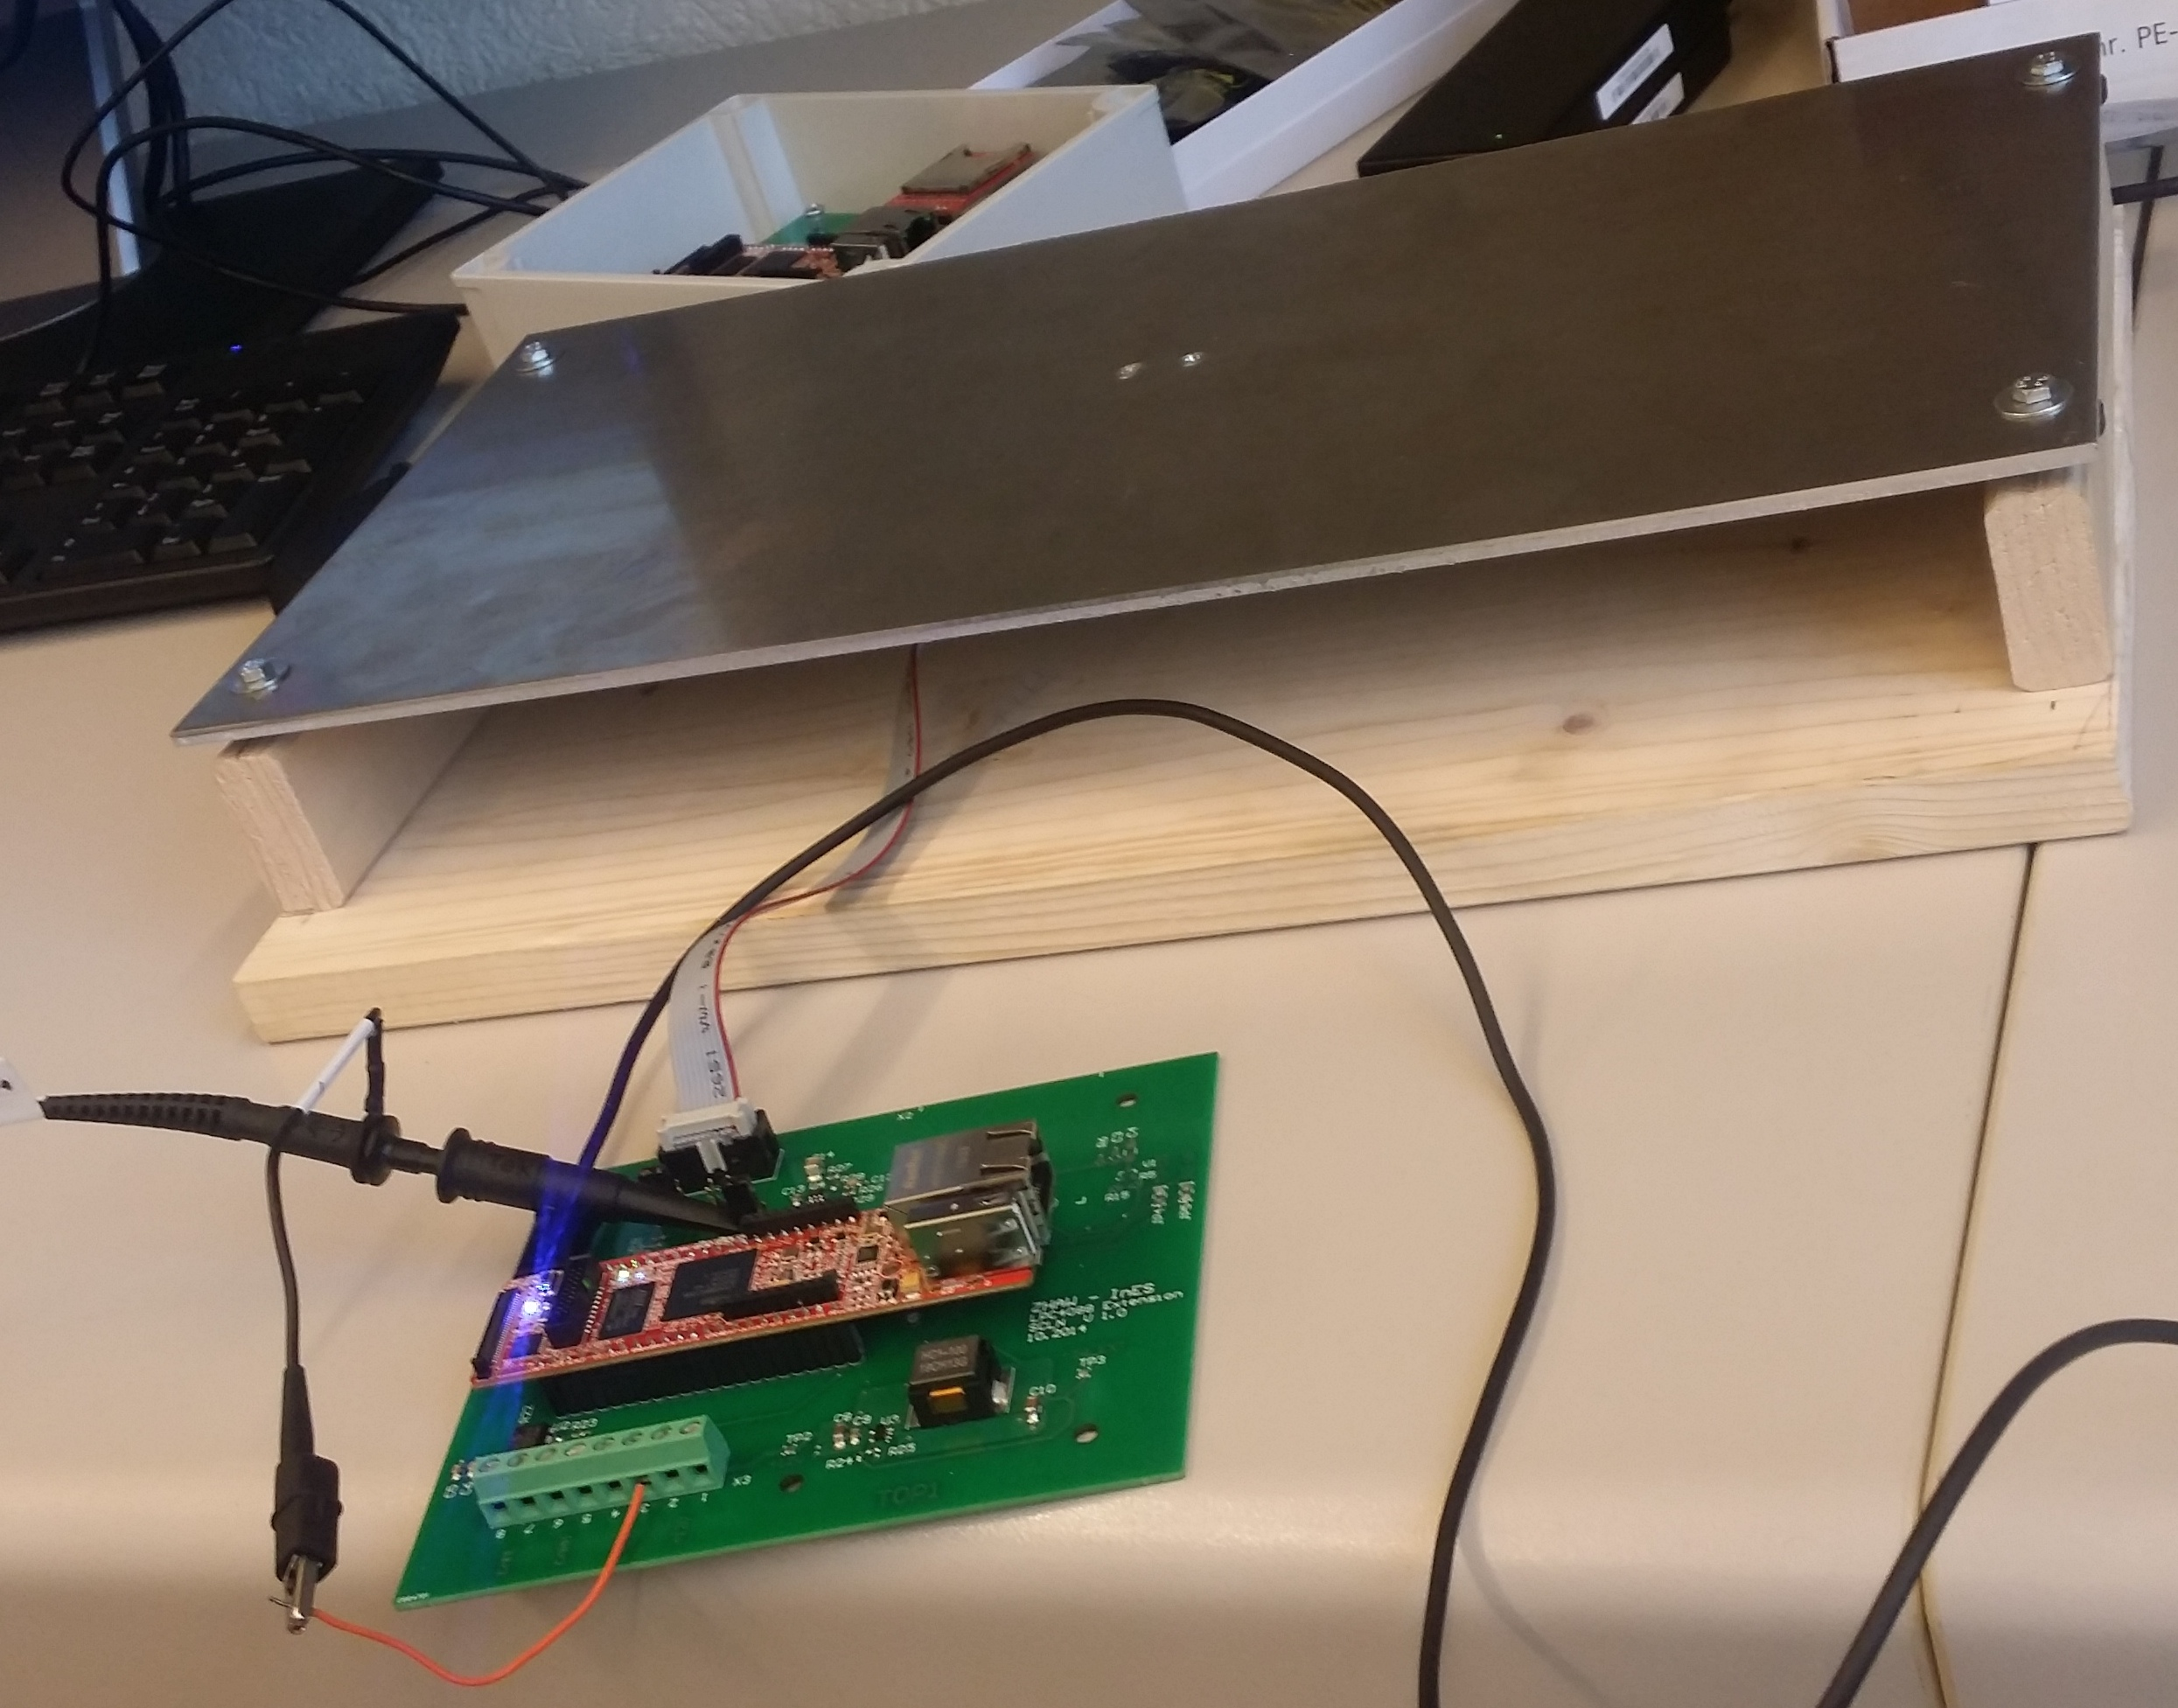
\includegraphics[width=0.8\textwidth]{images/fotos/testaufbau1.jpg}
	\caption{Übersicht des Testaufbaus.}
	\label{fig.testaufbau1}
\end{figure}

\begin{figure}
	\centering
		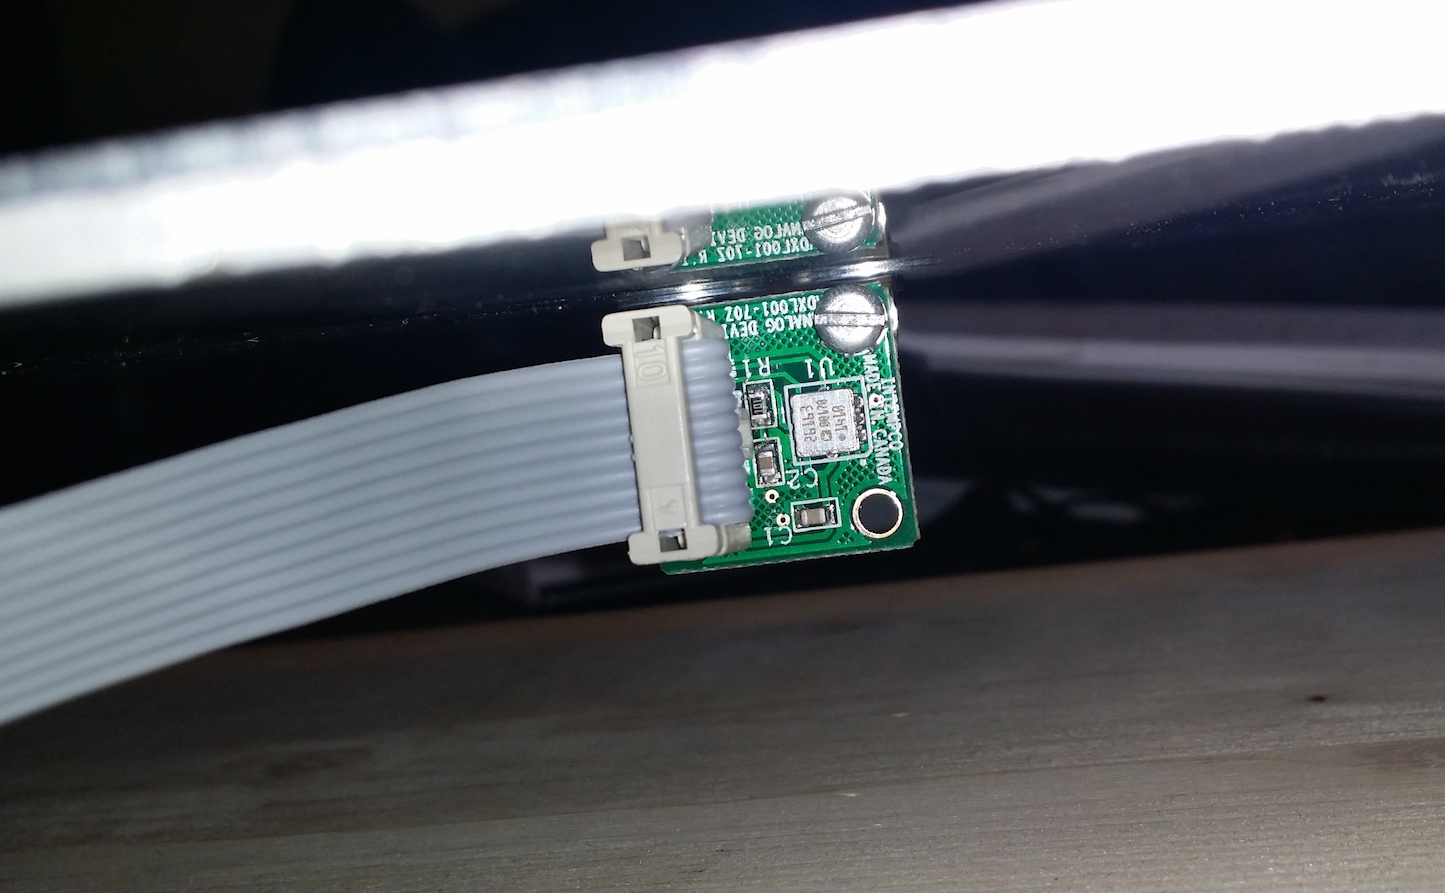
\includegraphics[width=0.8\textwidth]{images/fotos/testaufbau2.jpg}
	\caption{Montage des Sensors im Testaufbau.}
	\label{fig.testaufbau2}
\end{figure}

\section{Datenlogger}
\subsection{T110 Busmaster}
\paragraph{Aktionen} Die Messstation wird an die Stromversorgung angeschlossen.

\paragraph{Resultate} Der \gls{logger} übernimmt die Kontrolle über den CAN-Bus und vergibt jedem angeschlossenen Sensor die eindeutige CAN-ID aus der Konfigurationsdatei.

\paragraph{Testergebnis} Die \glspl{sensoreinh} haben die vordefinierte CAN-ID erhalten. Der Test ist erfüllt.

\subsection{T120 Sensorerkennung}
\paragraph{Aktionen} Eine neue \gls{sensoreinh} wird an die Messstation angeschlossen, deren Seriennummer nicht in der Konfigurationsdatei erfasst ist. Die Messstation wird an die Stromversorgung angeschlossen.

\paragraph{Resultate} Der \gls{logger} erkennt die neue \gls{sensoreinh} und teilt ihr eine eindeutige CAN-ID zu.

\paragraph{Testergebnis} Die \gls{sensoreinh} hat eine bisher unbenutzte, unreservierte CAN-ID erhalten. Der Test ist erfüllt.

\subsection{T130 Uhrzeit}
\paragraph{Aktionen} Die Uhrzeit wird im laufenden Betrieb richtig eingestellt. Die Messstation wird während mind. 12~Stunden in Betrieb gehalten.

\paragraph{Resultate} Die interne Uhrzeit weist nicht mehr als 2~Sekunden Fehlgang innert 12~Stunden auf.

\paragraph{Testergebnis} Bis zur Berichterstellung konnte dieser Test noch nicht durchgeführt werden.

\subsection{T140 Timestamp zurücksetzen}
\paragraph{Aktionen} Über die Konfigurationsschnittstelle wird der Befehl zum Zurücksetzen der \gls{timestamp}s in den \glspl{sensoreinh} gegeben.

\paragraph{Resultate} Alle \glspl{sensoreinh} führen den Befehl innert weniger Sekunden aus und senden ab dann die Ereignisse mit dem neuen \gls{timestamp}.

\paragraph{Testergebnis} Bis zur Berichterstellung konnte dieser Test noch nicht durchgeführt werden.

\subsection{T160 Schnittstelle zum Steuerrechner}
\paragraph{Aktionen} Ein \gls{compi} wird an die Konfigurationsschnittstelle angeschlossen und ein \gls{terminalemu} gestartet.

\paragraph{Resultate} Das Konfigurationsmenü erscheint in der Terminal-Emulation und kann über Tastatureingaben bedient werden.

Die Eingaben werden vom \gls{logger} ausgeführt und bei Bedarf an die \glspl{sensoreinh} kommuniziert.

\paragraph{Testergebnis} Das Konfigurationsmenü funktioniert wie vorgesehen. Die Einstellungen werden an die \glspl{sensoreinh} übertragen.

\subsection{T170 Steuerung Detail-Level}
\paragraph{Aktionen} Am \gls{logger} wird für eine \gls{sensoreinh} ein anderer Detail-Level eingestellt.

\paragraph{Resultate} Die \gls{sensoreinh} wechselt den Detail-Level bei der Übertragung neuer Ereignisse.

\paragraph{Testergebnis} Bis zur Berichterstellung konnte dieser Test noch nicht durchgeführt werden.

\subsection{T180 Daten sammeln und speichern}
\paragraph{Aktionen} Mehrere \glspl{sensoreinh} senden Ereignisdaten an den \gls{logger}. 

\paragraph{Resultate} Der \gls{logger} legt für jede \gls{sensoreinh} eine Datei an und speichert die Ereignisdaten in der richtigen Datei.

\paragraph{Testergebnis} Bis zur Berichterstellung konnte dieser Test noch nicht durchgeführt werden.


\section{Sensoreinheit}
\subsection{T400 Konfiguration}
\paragraph{Aktionen} Via Konfigurationsmenü des Datenloggers werden die Parameter des Sensors auf neue Werte gesetzt. 

\paragraph{Resultate} Die \gls{sensoreinh} übernimmt die neuen Einstellungen und passt die Ereigniserkennung entsprechend an.

\paragraph{Testergebnis} Die Konfiguration wurde erfolgreich auf die \gls{sensoreinh} übertragen. Die Konfiguration vor dem Test ist in Listing \ref{t400.1} gegeben, mit der Eingabe 99 werden alle Sensoren ausgewählt. Listings \ref{t400.2} und \ref{400.3} zeigen, wie der zu konfigurierende Parameter ausgewählt und der neue Wert eingegeben wird. Am \gls{logger} wird im Testmodus das Absenden einer CAN-Nachricht protokolliert, Listing \ref{t400.4}. Die \glspl{sensoreinh} geben im Testmodus ebenfalls eine Bestätigung aus (Listings \ref{t400.5} und \ref{t400.6}), wenn sie eine neue Konfiguration erhalten. Die Änderung des \gls{threshold}s wurde also von beiden Sensoren übernommen.

\begin{lstlisting}[caption=T400 Vorbedingung und Auswahl aller Sensoren, label=t400.1]
Listing sensor config
 Nr  SID  serial    fs  threshold baseline timeout detail     started?
 0)  2  061bfdf6   100        200     2047      30 sparse     started
 1)  3  15117738   100        150     2040      30 peaks only started
 #) Select a sensor from the list.
99) Select all sensors.
 0) cancel
 >
your entry was: 99
\end{lstlisting}

\begin{lstlisting}[caption=T400 Auswahl des Parameters, label=t400.2]
 1) set sampling rate
 2) set threshold value
 3) set baseline value
 4) set timeout
 5) set detail level
 6) start or stop recording
 0) exit
 >
your entry was: 2
\end{lstlisting}

\begin{lstlisting}[caption=T400 Eingabe des neuen \gls{threshold}s, label=t400.3]
 #) Enter threshold value.
baseline + threshold must not exceed 4096
and
baseline - threshold must not be below 0
 0) cancel
 >
your entry was: 250
\end{lstlisting}

\begin{lstlisting}[caption=T400 Sendeprotokoll am \gls{logger}, label=t400.4]
prepare message id: 5020101
OK
prepare message id: 50301001
OK
\end{lstlisting}

\begin{lstlisting}[caption=T400 Konfiguration aus Sensor 3, label=t400.5]
threshold fa   -> geaenderter Wert, von 150 (0x96) auf 250 (0xfa)
fsampling 64   -> wie zuvor, bei 100
timeout 1e     -> wie zuvor, bei 30
baseline 7f8   -> wie zuvor, bei 2040
\end{lstlisting}

\begin{lstlisting}[caption=T400 Konfiguration aus Sensor 2, label=t400.6]
threshold fa   -> geaenderter Wert, von 200 (0xc8) auf 250 (0xfa)
fsampling 64   -> wie zuvor, bei 100
timeout 1e     -> wie zuvor, bei 30
baseline 7ff   -> wie zuvor, bei 2047
\end{lstlisting}


\subsection{T410 Ereignisdetektion}
\paragraph{Aktionen} Die \gls{sensoreinh} ist im Messbetrieb. Am \gls{sensor} wird ein Einschlag simuliert, indem ein Objekt auf die Metallplatte geschlagen wird. 

\paragraph{Resultate} Am Ausgang des \gls{sensor}s misst ein Oszilloskop den Spannungsverlauf. Die so gemessene Referenzkurve wird mit den von der \gls{sensoreinh} ausgegebenen Daten verglichen.

\paragraph{Testergebnis} Bis zur Berichterstellung konnte dieser Test noch nicht durchgeführt werden.

\subsection{T430 Datenübertragung}
\paragraph{Aktionen} Mehrere Einschläge werden simuliert und mit einem Oszilloskop aufgezeichnet, um Referenzdaten zu haben.

\paragraph{Resultate} Die \gls{sensoreinh} überträgt die Daten von Test T410 fehlerfrei an den \gls{logger}.

\paragraph{Testergebnis} Bis zur Berichterstellung konnte dieser Test noch nicht durchgeführt werden.

\subsection{T450 Rohdatenaufzeichnung}
\paragraph{Aktionen} Eine \gls{sensoreinh} wird in den Rohdatenmodus versetzt.

\paragraph{Resultate} Die \gls{sensoreinh} zeichnet Rohdaten während 60 Sekunden ohne einen Puffer-Überlauf auf und überträgt die Daten an den \gls{logger}.

\paragraph{Testergebnis} Bis zur Berichterstellung konnte dieser Test noch nicht durchgeführt werden.

\section{Nichtfunktionale Tests}
\subsection{T710 Stromverbrauch}
\paragraph{Aktionen} Der Stromverbrauch der Messanlage mit dem \gls{logger} und drei \glspl{sensoreinh} wird gemessen. 

\paragraph{Resultate} Der Stromverbrauch sollte unter 3~Watt liegen.

\paragraph{Testergebnis} Ein \gls{logger} und zwei \gls{sensoreinh} haben einen Stromverbrauch von 